% generated by Plantuml 1.2022.7       
\definecolor{plantucolor0000}{RGB}{255,255,255}
\definecolor{plantucolor0001}{RGB}{24,24,24}
\definecolor{plantucolor0002}{RGB}{0,0,0}
\definecolor{plantucolor0003}{RGB}{226,226,240}
\definecolor{plantucolor0004}{RGB}{238,238,238}
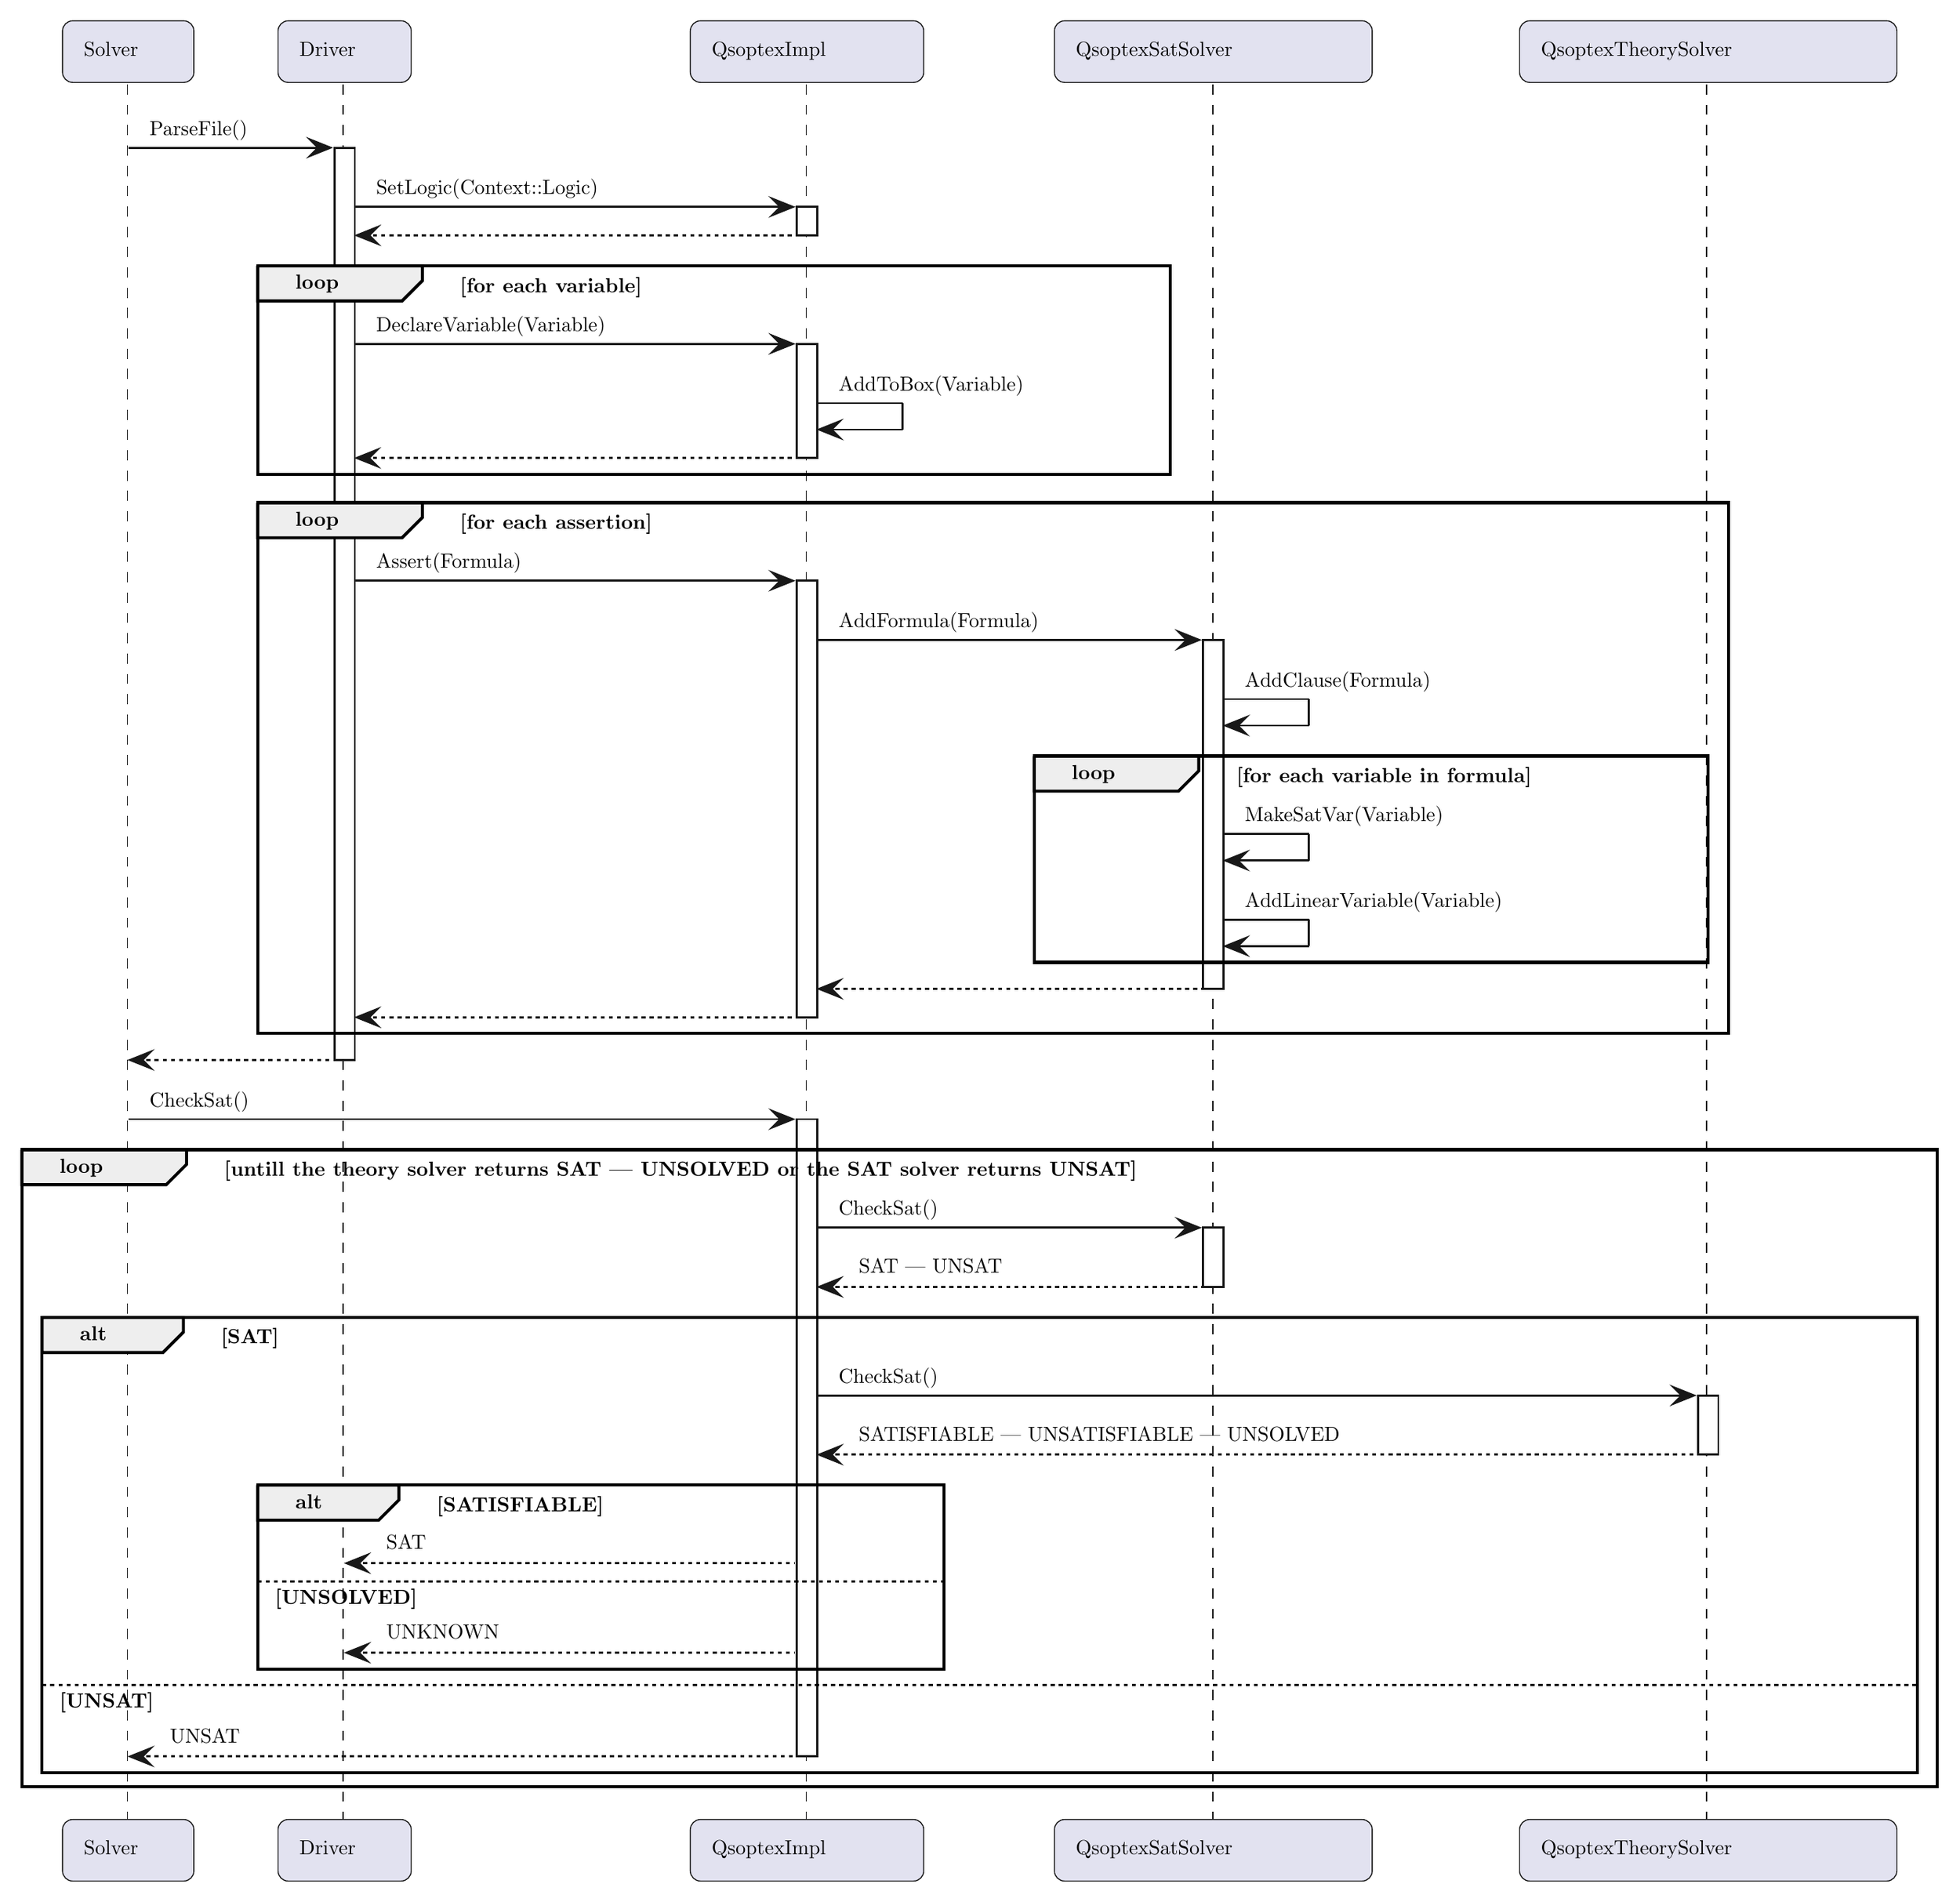
\begin{tikzpicture}[yscale=-1
,pstyle0/.style={color=plantucolor0001,fill=white,line width=1.0pt}
,pstyle1/.style={color=black,line width=1.5pt}
,pstyle2/.style={color=plantucolor0001,line width=0.5pt,dash pattern=on 5.0pt off 5.0pt}
,pstyle3/.style={color=plantucolor0001,fill=plantucolor0003,line width=0.5pt}
,pstyle4/.style={color=plantucolor0001,fill=plantucolor0001,line width=1.0pt}
,pstyle5/.style={color=plantucolor0001,line width=1.0pt}
,pstyle6/.style={color=plantucolor0001,line width=1.0pt,dash pattern=on 2.0pt off 2.0pt}
,pstyle7/.style={color=black,fill=plantucolor0004,line width=1.5pt}
,pstyle8/.style={color=black,line width=1.0pt,dash pattern=on 2.0pt off 2.0pt}
]
\draw[pstyle0] (163.7662pt,67.4297pt) rectangle (173.7662pt,516.3096pt);
\draw[pstyle0] (391.1996pt,96.5625pt) rectangle (401.1996pt,110.5625pt);
\draw[pstyle0] (391.1996pt,163.9678pt) rectangle (401.1996pt,220.1006pt);
\draw[pstyle0] (391.1996pt,280.5059pt) rectangle (401.1996pt,495.3096pt);
\draw[pstyle0] (391.1996pt,545.4424pt) rectangle (401.1996pt,859.0352pt);
\draw[pstyle0] (591.0547pt,309.6387pt) rectangle (601.0547pt,481.3096pt);
\draw[pstyle0] (591.0547pt,598.8477pt) rectangle (601.0547pt,627.9805pt);
\draw[pstyle0] (834.4601pt,681.3857pt) rectangle (844.4601pt,710.5186pt);
\draw[pstyle1] (126.0107pt,125.5625pt) rectangle (574.8347pt,228.1006pt);
\draw[pstyle1] (126.0107pt,242.1006pt) rectangle (849.4601pt,503.3096pt);
\draw[pstyle1] (507.8947pt,366.7715pt) rectangle (839.4601pt,468.3096pt);
\draw[pstyle1] (10pt,560.4424pt) rectangle (952.239pt,874.0352pt);
\draw[pstyle1] (20pt,642.9805pt) rectangle (942.239pt,867.0352pt);
\draw[pstyle1] (126.0107pt,725.5186pt) rectangle (463.5996pt,815.9795pt);
\draw[pstyle2] (62pt,36.2969pt) -- (62pt,891.0352pt);
\draw[pstyle2] (168.0107pt,36.2969pt) -- (168.0107pt,891.0352pt);
\draw[pstyle2] (395.7996pt,36.2969pt) -- (395.7996pt,891.0352pt);
\draw[pstyle2] (595.8947pt,36.2969pt) -- (595.8947pt,891.0352pt);
\draw[pstyle2] (838.6813pt,36.2969pt) -- (838.6813pt,891.0352pt);
\draw[pstyle3] (30pt,10pt) arc (180:270:5pt) -- (35pt,5pt) -- (89.6182pt,5pt) arc (270:360:5pt) -- (94.6182pt,10pt) -- (94.6182pt,30.2969pt) arc (0:90:5pt) -- (89.6182pt,35.2969pt) -- (35pt,35.2969pt) arc (90:180:5pt) -- (30pt,30.2969pt) -- cycle;
\node at (37pt,12pt)[below right,color=black]{Solver};
\draw[pstyle3] (30pt,895.0352pt) arc (180:270:5pt) -- (35pt,890.0352pt) -- (89.6182pt,890.0352pt) arc (270:360:5pt) -- (94.6182pt,895.0352pt) -- (94.6182pt,915.332pt) arc (0:90:5pt) -- (89.6182pt,920.332pt) -- (35pt,920.332pt) arc (90:180:5pt) -- (30pt,915.332pt) -- cycle;
\node at (37pt,897.0352pt)[below right,color=black]{Solver};
\draw[pstyle3] (136.0107pt,10pt) arc (180:270:5pt) -- (141.0107pt,5pt) -- (196.5218pt,5pt) arc (270:360:5pt) -- (201.5218pt,10pt) -- (201.5218pt,30.2969pt) arc (0:90:5pt) -- (196.5218pt,35.2969pt) -- (141.0107pt,35.2969pt) arc (90:180:5pt) -- (136.0107pt,30.2969pt) -- cycle;
\node at (143.0107pt,12pt)[below right,color=black]{Driver};
\draw[pstyle3] (136.0107pt,895.0352pt) arc (180:270:5pt) -- (141.0107pt,890.0352pt) -- (196.5218pt,890.0352pt) arc (270:360:5pt) -- (201.5218pt,895.0352pt) -- (201.5218pt,915.332pt) arc (0:90:5pt) -- (196.5218pt,920.332pt) -- (141.0107pt,920.332pt) arc (90:180:5pt) -- (136.0107pt,915.332pt) -- cycle;
\node at (143.0107pt,897.0352pt)[below right,color=black]{Driver};
\draw[pstyle3] (338.7996pt,10pt) arc (180:270:5pt) -- (343.7996pt,5pt) -- (448.5996pt,5pt) arc (270:360:5pt) -- (453.5996pt,10pt) -- (453.5996pt,30.2969pt) arc (0:90:5pt) -- (448.5996pt,35.2969pt) -- (343.7996pt,35.2969pt) arc (90:180:5pt) -- (338.7996pt,30.2969pt) -- cycle;
\node at (345.7996pt,12pt)[below right,color=black]{QsoptexImpl};
\draw[pstyle3] (338.7996pt,895.0352pt) arc (180:270:5pt) -- (343.7996pt,890.0352pt) -- (448.5996pt,890.0352pt) arc (270:360:5pt) -- (453.5996pt,895.0352pt) -- (453.5996pt,915.332pt) arc (0:90:5pt) -- (448.5996pt,920.332pt) -- (343.7996pt,920.332pt) arc (90:180:5pt) -- (338.7996pt,915.332pt) -- cycle;
\node at (345.7996pt,897.0352pt)[below right,color=black]{QsoptexImpl};
\draw[pstyle3] (517.8947pt,10pt) arc (180:270:5pt) -- (522.8947pt,5pt) -- (669.2147pt,5pt) arc (270:360:5pt) -- (674.2147pt,10pt) -- (674.2147pt,30.2969pt) arc (0:90:5pt) -- (669.2147pt,35.2969pt) -- (522.8947pt,35.2969pt) arc (90:180:5pt) -- (517.8947pt,30.2969pt) -- cycle;
\node at (524.8947pt,12pt)[below right,color=black]{QsoptexSatSolver};
\draw[pstyle3] (517.8947pt,895.0352pt) arc (180:270:5pt) -- (522.8947pt,890.0352pt) -- (669.2147pt,890.0352pt) arc (270:360:5pt) -- (674.2147pt,895.0352pt) -- (674.2147pt,915.332pt) arc (0:90:5pt) -- (669.2147pt,920.332pt) -- (522.8947pt,920.332pt) arc (90:180:5pt) -- (517.8947pt,915.332pt) -- cycle;
\node at (524.8947pt,897.0352pt)[below right,color=black]{QsoptexSatSolver};
\draw[pstyle3] (746.6813pt,10pt) arc (180:270:5pt) -- (751.6813pt,5pt) -- (927.239pt,5pt) arc (270:360:5pt) -- (932.239pt,10pt) -- (932.239pt,30.2969pt) arc (0:90:5pt) -- (927.239pt,35.2969pt) -- (751.6813pt,35.2969pt) arc (90:180:5pt) -- (746.6813pt,30.2969pt) -- cycle;
\node at (753.6813pt,12pt)[below right,color=black]{QsoptexTheorySolver};
\draw[pstyle3] (746.6813pt,895.0352pt) arc (180:270:5pt) -- (751.6813pt,890.0352pt) -- (927.239pt,890.0352pt) arc (270:360:5pt) -- (932.239pt,895.0352pt) -- (932.239pt,915.332pt) arc (0:90:5pt) -- (927.239pt,920.332pt) -- (751.6813pt,920.332pt) arc (90:180:5pt) -- (746.6813pt,915.332pt) -- cycle;
\node at (753.6813pt,897.0352pt)[below right,color=black]{QsoptexTheorySolver};
\draw[pstyle0] (163.7662pt,67.4297pt) rectangle (173.7662pt,516.3096pt);
\draw[pstyle0] (391.1996pt,96.5625pt) rectangle (401.1996pt,110.5625pt);
\draw[pstyle0] (391.1996pt,163.9678pt) rectangle (401.1996pt,220.1006pt);
\draw[pstyle0] (391.1996pt,280.5059pt) rectangle (401.1996pt,495.3096pt);
\draw[pstyle0] (391.1996pt,545.4424pt) rectangle (401.1996pt,859.0352pt);
\draw[pstyle0] (591.0547pt,309.6387pt) rectangle (601.0547pt,481.3096pt);
\draw[pstyle0] (591.0547pt,598.8477pt) rectangle (601.0547pt,627.9805pt);
\draw[pstyle0] (834.4601pt,681.3857pt) rectangle (844.4601pt,710.5186pt);
\draw[pstyle4] (151.7662pt,63.4297pt) -- (161.7662pt,67.4297pt) -- (151.7662pt,71.4297pt) -- (155.7662pt,67.4297pt) -- cycle;
\draw[pstyle5] (62.3091pt,67.4297pt) -- (157.7662pt,67.4297pt);
\node at (69.3091pt,50.2969pt)[below right,color=black]{ParseFile()};
\draw[pstyle4] (379.1996pt,92.5625pt) -- (389.1996pt,96.5625pt) -- (379.1996pt,100.5625pt) -- (383.1996pt,96.5625pt) -- cycle;
\draw[pstyle5] (173.7662pt,96.5625pt) -- (385.1996pt,96.5625pt);
\node at (180.7662pt,79.4297pt)[below right,color=black]{SetLogic(Context::Logic)};
\draw[pstyle4] (184.7662pt,106.5625pt) -- (174.7662pt,110.5625pt) -- (184.7662pt,114.5625pt) -- (180.7662pt,110.5625pt) -- cycle;
\draw[pstyle6] (178.7662pt,110.5625pt) -- (395.1996pt,110.5625pt);
\draw[pstyle7] (126.0107pt,125.5625pt) -- (207.0107pt,125.5625pt) -- (207.0107pt,132.835pt) -- (197.0107pt,142.835pt) -- (126.0107pt,142.835pt) -- (126.0107pt,125.5625pt);
\draw[pstyle1] (126.0107pt,125.5625pt) rectangle (574.8347pt,228.1006pt);
\node at (141.0107pt,126.5625pt)[below right,color=black]{\textbf{loop}};
\node at (222.0107pt,127.5625pt)[below right,color=black]{\textbf{[for each variable]}};
\draw[pstyle4] (379.1996pt,159.9678pt) -- (389.1996pt,163.9678pt) -- (379.1996pt,167.9678pt) -- (383.1996pt,163.9678pt) -- cycle;
\draw[pstyle5] (173.7662pt,163.9678pt) -- (385.1996pt,163.9678pt);
\node at (180.7662pt,146.835pt)[below right,color=black]{DeclareVariable(Variable)};
\draw[pstyle5] (401.1996pt,193.1006pt) -- (443.1996pt,193.1006pt);
\draw[pstyle5] (443.1996pt,193.1006pt) -- (443.1996pt,206.1006pt);
\draw[pstyle5] (402.1996pt,206.1006pt) -- (443.1996pt,206.1006pt);
\draw[pstyle4] (412.1996pt,202.1006pt) -- (402.1996pt,206.1006pt) -- (412.1996pt,210.1006pt) -- (408.1996pt,206.1006pt) -- cycle;
\node at (408.1996pt,175.9678pt)[below right,color=black]{AddToBox(Variable)};
\draw[pstyle4] (184.7662pt,216.1006pt) -- (174.7662pt,220.1006pt) -- (184.7662pt,224.1006pt) -- (180.7662pt,220.1006pt) -- cycle;
\draw[pstyle6] (178.7662pt,220.1006pt) -- (395.1996pt,220.1006pt);
\draw[pstyle7] (126.0107pt,242.1006pt) -- (207.0107pt,242.1006pt) -- (207.0107pt,249.373pt) -- (197.0107pt,259.373pt) -- (126.0107pt,259.373pt) -- (126.0107pt,242.1006pt);
\draw[pstyle1] (126.0107pt,242.1006pt) rectangle (849.4601pt,503.3096pt);
\node at (141.0107pt,243.1006pt)[below right,color=black]{\textbf{loop}};
\node at (222.0107pt,244.1006pt)[below right,color=black]{\textbf{[for each assertion]}};
\draw[pstyle4] (379.1996pt,276.5059pt) -- (389.1996pt,280.5059pt) -- (379.1996pt,284.5059pt) -- (383.1996pt,280.5059pt) -- cycle;
\draw[pstyle5] (173.7662pt,280.5059pt) -- (385.1996pt,280.5059pt);
\node at (180.7662pt,263.373pt)[below right,color=black]{Assert(Formula)};
\draw[pstyle4] (579.0547pt,305.6387pt) -- (589.0547pt,309.6387pt) -- (579.0547pt,313.6387pt) -- (583.0547pt,309.6387pt) -- cycle;
\draw[pstyle5] (401.1996pt,309.6387pt) -- (585.0547pt,309.6387pt);
\node at (408.1996pt,292.5059pt)[below right,color=black]{AddFormula(Formula)};
\draw[pstyle5] (601.0547pt,338.7715pt) -- (643.0547pt,338.7715pt);
\draw[pstyle5] (643.0547pt,338.7715pt) -- (643.0547pt,351.7715pt);
\draw[pstyle5] (602.0547pt,351.7715pt) -- (643.0547pt,351.7715pt);
\draw[pstyle4] (612.0547pt,347.7715pt) -- (602.0547pt,351.7715pt) -- (612.0547pt,355.7715pt) -- (608.0547pt,351.7715pt) -- cycle;
\node at (608.0547pt,321.6387pt)[below right,color=black]{AddClause(Formula)};
\draw[pstyle7] (507.8947pt,366.7715pt) -- (588.8947pt,366.7715pt) -- (588.8947pt,374.0439pt) -- (578.8947pt,384.0439pt) -- (507.8947pt,384.0439pt) -- (507.8947pt,366.7715pt);
\draw[pstyle1] (507.8947pt,366.7715pt) rectangle (839.4601pt,468.3096pt);
\node at (522.8947pt,367.7715pt)[below right,color=black]{\textbf{loop}};
\node at (603.8947pt,368.7715pt)[below right,color=black]{\textbf{[for each variable in formula]}};
\draw[pstyle5] (601.0547pt,405.1768pt) -- (643.0547pt,405.1768pt);
\draw[pstyle5] (643.0547pt,405.1768pt) -- (643.0547pt,418.1768pt);
\draw[pstyle5] (602.0547pt,418.1768pt) -- (643.0547pt,418.1768pt);
\draw[pstyle4] (612.0547pt,414.1768pt) -- (602.0547pt,418.1768pt) -- (612.0547pt,422.1768pt) -- (608.0547pt,418.1768pt) -- cycle;
\node at (608.0547pt,388.0439pt)[below right,color=black]{MakeSatVar(Variable)};
\draw[pstyle5] (601.0547pt,447.3096pt) -- (643.0547pt,447.3096pt);
\draw[pstyle5] (643.0547pt,447.3096pt) -- (643.0547pt,460.3096pt);
\draw[pstyle5] (602.0547pt,460.3096pt) -- (643.0547pt,460.3096pt);
\draw[pstyle4] (612.0547pt,456.3096pt) -- (602.0547pt,460.3096pt) -- (612.0547pt,464.3096pt) -- (608.0547pt,460.3096pt) -- cycle;
\node at (608.0547pt,430.1768pt)[below right,color=black]{AddLinearVariable(Variable)};
\draw[pstyle4] (412.1996pt,477.3096pt) -- (402.1996pt,481.3096pt) -- (412.1996pt,485.3096pt) -- (408.1996pt,481.3096pt) -- cycle;
\draw[pstyle6] (406.1996pt,481.3096pt) -- (595.0547pt,481.3096pt);
\draw[pstyle4] (184.7662pt,491.3096pt) -- (174.7662pt,495.3096pt) -- (184.7662pt,499.3096pt) -- (180.7662pt,495.3096pt) -- cycle;
\draw[pstyle6] (178.7662pt,495.3096pt) -- (395.1996pt,495.3096pt);
\draw[pstyle4] (73.3091pt,512.3096pt) -- (63.3091pt,516.3096pt) -- (73.3091pt,520.3096pt) -- (69.3091pt,516.3096pt) -- cycle;
\draw[pstyle6] (67.3091pt,516.3096pt) -- (167.7662pt,516.3096pt);
\draw[pstyle4] (379.1996pt,541.4424pt) -- (389.1996pt,545.4424pt) -- (379.1996pt,549.4424pt) -- (383.1996pt,545.4424pt) -- cycle;
\draw[pstyle5] (62.3091pt,545.4424pt) -- (385.1996pt,545.4424pt);
\node at (69.3091pt,528.3096pt)[below right,color=black]{CheckSat()};
\draw[pstyle7] (10pt,560.4424pt) -- (91pt,560.4424pt) -- (91pt,567.7148pt) -- (81pt,577.7148pt) -- (10pt,577.7148pt) -- (10pt,560.4424pt);
\draw[pstyle1] (10pt,560.4424pt) rectangle (952.239pt,874.0352pt);
\node at (25pt,561.4424pt)[below right,color=black]{\textbf{loop}};
\node at (106pt,562.4424pt)[below right,color=black]{\textbf{[untill the theory solver returns SAT | UNSOLVED or the SAT solver returns UNSAT]}};
\draw[pstyle4] (579.0547pt,594.8477pt) -- (589.0547pt,598.8477pt) -- (579.0547pt,602.8477pt) -- (583.0547pt,598.8477pt) -- cycle;
\draw[pstyle5] (401.1996pt,598.8477pt) -- (585.0547pt,598.8477pt);
\node at (408.1996pt,581.7148pt)[below right,color=black]{CheckSat()};
\draw[pstyle4] (412.1996pt,623.9805pt) -- (402.1996pt,627.9805pt) -- (412.1996pt,631.9805pt) -- (408.1996pt,627.9805pt) -- cycle;
\draw[pstyle6] (406.1996pt,627.9805pt) -- (595.0547pt,627.9805pt);
\node at (418.1996pt,610.8477pt)[below right,color=black]{SAT | UNSAT};
\draw[pstyle7] (20pt,642.9805pt) -- (89.4381pt,642.9805pt) -- (89.4381pt,650.2529pt) -- (79.4381pt,660.2529pt) -- (20pt,660.2529pt) -- (20pt,642.9805pt);
\draw[pstyle1] (20pt,642.9805pt) rectangle (942.239pt,867.0352pt);
\node at (35pt,643.9805pt)[below right,color=black]{\textbf{alt}};
\node at (104.4381pt,644.9805pt)[below right,color=black]{\textbf{[SAT]}};
\draw[pstyle4] (822.4601pt,677.3857pt) -- (832.4601pt,681.3857pt) -- (822.4601pt,685.3857pt) -- (826.4601pt,681.3857pt) -- cycle;
\draw[pstyle5] (401.1996pt,681.3857pt) -- (828.4601pt,681.3857pt);
\node at (408.1996pt,664.2529pt)[below right,color=black]{CheckSat()};
\draw[pstyle4] (412.1996pt,706.5186pt) -- (402.1996pt,710.5186pt) -- (412.1996pt,714.5186pt) -- (408.1996pt,710.5186pt) -- cycle;
\draw[pstyle6] (406.1996pt,710.5186pt) -- (838.4601pt,710.5186pt);
\node at (418.1996pt,693.3857pt)[below right,color=black]{SATISFIABLE | UNSATISFIABLE | UNSOLVED};
\draw[pstyle7] (126.0107pt,725.5186pt) -- (195.4488pt,725.5186pt) -- (195.4488pt,732.791pt) -- (185.4488pt,742.791pt) -- (126.0107pt,742.791pt) -- (126.0107pt,725.5186pt);
\draw[pstyle1] (126.0107pt,725.5186pt) rectangle (463.5996pt,815.9795pt);
\node at (141.0107pt,726.5186pt)[below right,color=black]{\textbf{alt}};
\node at (210.4488pt,727.5186pt)[below right,color=black]{\textbf{[SATISFIABLE]}};
\draw[pstyle4] (179.7662pt,759.9238pt) -- (169.7662pt,763.9238pt) -- (179.7662pt,767.9238pt) -- (175.7662pt,763.9238pt) -- cycle;
\draw[pstyle6] (173.7662pt,763.9238pt) -- (390.1996pt,763.9238pt);
\node at (185.7662pt,746.791pt)[below right,color=black]{SAT};
\draw[pstyle8] (126.0107pt,772.9238pt) -- (463.5996pt,772.9238pt);
\node at (131.0107pt,772.9238pt)[below right,color=black]{\textbf{[UNSOLVED]}};
\draw[pstyle4] (179.7662pt,803.9795pt) -- (169.7662pt,807.9795pt) -- (179.7662pt,811.9795pt) -- (175.7662pt,807.9795pt) -- cycle;
\draw[pstyle6] (173.7662pt,807.9795pt) -- (390.1996pt,807.9795pt);
\node at (185.7662pt,790.8467pt)[below right,color=black]{UNKNOWN};
\draw[pstyle8] (20pt,823.9795pt) -- (942.239pt,823.9795pt);
\node at (25pt,823.9795pt)[below right,color=black]{\textbf{[UNSAT]}};
\draw[pstyle4] (73.3091pt,855.0352pt) -- (63.3091pt,859.0352pt) -- (73.3091pt,863.0352pt) -- (69.3091pt,859.0352pt) -- cycle;
\draw[pstyle6] (67.3091pt,859.0352pt) -- (395.1996pt,859.0352pt);
\node at (79.3091pt,841.9023pt)[below right,color=black]{UNSAT};
\end{tikzpicture}
